\documentclass{standalone}
\usepackage{tikz}
\usetikzlibrary{patterns, positioning}


\begin{document}
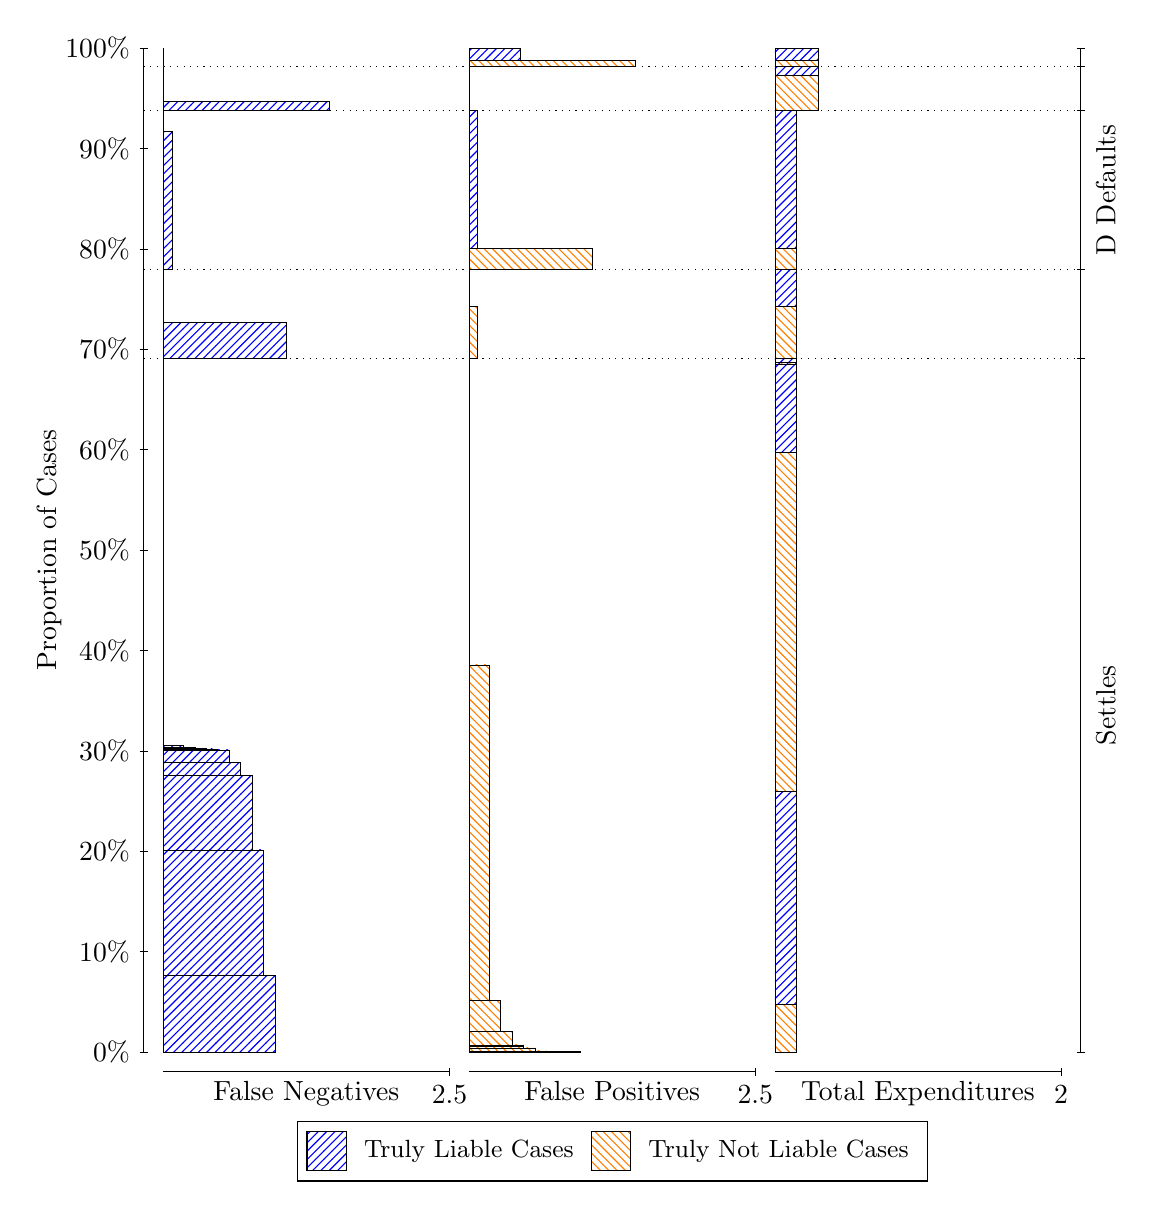
\begin{tikzpicture}
\draw[black, very thin] (1.5,1.75) -- (1.5,14.5);
\node[rotate=90, text=black, anchor=center] at (0.3, 8.125) {Proportion of Cases};
\draw[black, very thin] (1.45,1.75) -- (1.55,1.75);
\node[text=black, anchor=east] at (1.45, 1.75) {0\%};
\draw[black, very thin] (1.45,3.025) -- (1.55,3.025);
\node[text=black, anchor=east] at (1.45, 3.025) {10\%};
\draw[black, very thin] (1.45,4.3) -- (1.55,4.3);
\node[text=black, anchor=east] at (1.45, 4.3) {20\%};
\draw[black, very thin] (1.45,5.575) -- (1.55,5.575);
\node[text=black, anchor=east] at (1.45, 5.575) {30\%};
\draw[black, very thin] (1.45,6.85) -- (1.55,6.85);
\node[text=black, anchor=east] at (1.45, 6.85) {40\%};
\draw[black, very thin] (1.45,8.125) -- (1.55,8.125);
\node[text=black, anchor=east] at (1.45, 8.125) {50\%};
\draw[black, very thin] (1.45,9.4) -- (1.55,9.4);
\node[text=black, anchor=east] at (1.45, 9.4) {60\%};
\draw[black, very thin] (1.45,10.675) -- (1.55,10.675);
\node[text=black, anchor=east] at (1.45, 10.675) {70\%};
\draw[black, very thin] (1.45,11.95) -- (1.55,11.95);
\node[text=black, anchor=east] at (1.45, 11.95) {80\%};
\draw[black, very thin] (1.45,13.225) -- (1.55,13.225);
\node[text=black, anchor=east] at (1.45, 13.225) {90\%};
\draw[black, very thin] (1.45,14.5) -- (1.55,14.5);
\node[text=black, anchor=east] at (1.45, 14.5) {100\%};

\draw[black, very thin] (13.4,1.75) -- (13.4,14.5);
\draw[black, very thin] (13.35,1.75) -- (13.45,1.75);
\node[anchor=west] at (13.35, 1.75) {};
\draw[black, very thin] (13.35,10.556) -- (13.45,10.556);
\node[anchor=west] at (13.35, 10.556) {};
\draw[black, very thin] (13.35,11.687) -- (13.45,11.687);
\node[anchor=west] at (13.35, 11.687) {};
\draw[black, very thin] (13.35,13.707) -- (13.45,13.707);
\node[anchor=west] at (13.35, 13.707) {};
\draw[black, very thin] (13.35,14.268) -- (13.45,14.268);
\node[anchor=west] at (13.35, 14.268) {};
\draw[black, very thin] (13.35,14.5) -- (13.45,14.5);
\node[anchor=west] at (13.35, 14.5) {};

\draw[black, very thin, pattern color=blue, pattern=north east lines] (1.75,1.75) rectangle (3.167,2.7196);
\draw[black, very thin, pattern color=blue, pattern=north east lines] (1.75,2.7196) rectangle (3.0217,4.3157);
\draw[black, very thin, pattern color=blue, pattern=north east lines] (1.75,4.3157) rectangle (2.8763,5.2653);
\draw[black, very thin, pattern color=blue, pattern=north east lines] (1.75,5.2653) rectangle (2.731,5.4268);
\draw[black, very thin, pattern color=blue, pattern=north east lines] (1.75,5.4268) rectangle (2.5857,5.5871);
\draw[black, very thin, pattern color=blue, pattern=north east lines] (1.75,5.5871) rectangle (2.4403,5.5996);
\draw[black, very thin, pattern color=blue, pattern=north east lines] (1.75,5.5996) rectangle (2.295,5.6101);
\draw[black, very thin, pattern color=blue, pattern=north east lines] (1.75,5.6101) rectangle (2.1497,5.6161);
\draw[black, very thin, pattern color=blue, pattern=north east lines] (1.75,5.6161) rectangle (2.0043,5.639);
\draw[black, very thin, pattern color=orange, pattern=north west lines] (1.75,5.639) rectangle (1.75,10.556);
\draw[black, very thin, pattern color=blue, pattern=north east lines] (1.75,10.556) rectangle (3.3123,11.02);
\draw[black, very thin, pattern color=orange, pattern=north west lines] (1.75,11.02) rectangle (1.75,11.687);
\draw[black, very thin, pattern color=blue, pattern=north east lines] (1.75,11.687) rectangle (1.859,13.443);
\draw[black, very thin, pattern color=orange, pattern=north west lines] (1.75,13.443) rectangle (1.75,13.707);
\draw[black, very thin, pattern color=blue, pattern=north east lines] (1.75,13.707) rectangle (3.8573,13.819);
\draw[black, very thin, pattern color=orange, pattern=north west lines] (1.75,13.819) rectangle (1.75,14.268);
\draw[black, very thin, pattern color=orange, pattern=north west lines] (1.75,14.268) rectangle (1.75,14.347);
\draw[black, very thin, pattern color=blue, pattern=north east lines] (1.75,14.347) rectangle (1.75,14.5);
\draw[black, very thin, pattern color=orange, pattern=north west lines] (5.6333,1.75) rectangle (7.0503,1.7555);
\draw[black, very thin, pattern color=orange, pattern=north west lines] (5.6333,1.7555) rectangle (6.905,1.7569);
\draw[black, very thin, pattern color=orange, pattern=north west lines] (5.6333,1.7569) rectangle (6.7597,1.7601);
\draw[black, very thin, pattern color=orange, pattern=north west lines] (5.6333,1.7601) rectangle (6.6143,1.7643);
\draw[black, very thin, pattern color=orange, pattern=north west lines] (5.6333,1.7643) rectangle (6.469,1.8029);
\draw[black, very thin, pattern color=orange, pattern=north west lines] (5.6333,1.8029) rectangle (6.3237,1.8216);
\draw[black, very thin, pattern color=orange, pattern=north west lines] (5.6333,1.8216) rectangle (6.3237,1.8393);
\draw[black, very thin, pattern color=orange, pattern=north west lines] (5.6333,1.8393) rectangle (6.1783,2.01);
\draw[black, very thin, pattern color=orange, pattern=north west lines] (5.6333,2.01) rectangle (6.033,2.4055);
\draw[black, very thin, pattern color=orange, pattern=north west lines] (5.6333,2.4055) rectangle (5.8877,6.667);
\draw[black, very thin, pattern color=blue, pattern=north east lines] (5.6333,6.667) rectangle (5.6333,10.556);
\draw[black, very thin, pattern color=orange, pattern=north west lines] (5.6333,10.556) rectangle (5.7423,11.222);
\draw[black, very thin, pattern color=blue, pattern=north east lines] (5.6333,11.222) rectangle (5.6333,11.687);
\draw[black, very thin, pattern color=orange, pattern=north west lines] (5.6333,11.687) rectangle (7.1957,11.951);
\draw[black, very thin, pattern color=blue, pattern=north east lines] (5.6333,11.951) rectangle (5.7423,13.707);
\draw[black, very thin, pattern color=orange, pattern=north west lines] (5.6333,13.707) rectangle (5.6333,14.155);
\draw[black, very thin, pattern color=blue, pattern=north east lines] (5.6333,14.155) rectangle (5.6333,14.268);
\draw[black, very thin, pattern color=orange, pattern=north west lines] (5.6333,14.268) rectangle (7.7407,14.347);
\draw[black, very thin, pattern color=blue, pattern=north east lines] (5.6333,14.347) rectangle (6.2873,14.5);
\draw[black, very thin, pattern color=orange, pattern=north west lines] (9.5167,1.75) rectangle (9.7892,2.3526);
\draw[black, very thin, pattern color=blue, pattern=north east lines] (9.5167,2.3526) rectangle (9.7892,5.0598);
\draw[black, very thin, pattern color=orange, pattern=north west lines] (9.5167,5.0598) rectangle (9.7892,9.3598);
\draw[black, very thin, pattern color=blue, pattern=north east lines] (9.5167,9.3598) rectangle (9.7892,10.49);
\draw[black, very thin, pattern color=orange, pattern=north west lines] (9.5167,10.49) rectangle (9.7892,10.504);
\draw[black, very thin, pattern color=blue, pattern=north east lines] (9.5167,10.504) rectangle (9.7892,10.556);
\draw[black, very thin, pattern color=orange, pattern=north west lines] (9.5167,10.556) rectangle (9.7892,11.222);
\draw[black, very thin, pattern color=blue, pattern=north east lines] (9.5167,11.222) rectangle (9.7892,11.687);
\draw[black, very thin, pattern color=orange, pattern=north west lines] (9.5167,11.687) rectangle (9.7892,11.951);
\draw[black, very thin, pattern color=blue, pattern=north east lines] (9.5167,11.951) rectangle (9.7892,13.707);
\draw[black, very thin, pattern color=orange, pattern=north west lines] (9.5167,13.707) rectangle (10.062,14.155);
\draw[black, very thin, pattern color=blue, pattern=north east lines] (9.5167,14.155) rectangle (10.062,14.268);
\draw[black, very thin, pattern color=orange, pattern=north west lines] (9.5167,14.268) rectangle (10.062,14.347);
\draw[black, very thin, pattern color=blue, pattern=north east lines] (9.5167,14.347) rectangle (10.062,14.5);
\draw[black, dotted] (1.5,10.556) -- (13.4,10.556);
\draw[black, dotted] (1.5,11.687) -- (13.4,11.687);
\draw[black, dotted] (1.5,13.707) -- (13.4,13.707);
\draw[black, dotted] (1.5,14.268) -- (13.4,14.268);
\draw[black, very thin] (1.75,1.5) -- (5.3833,1.5);
\node[text=black, anchor=north] at (3.5667, 1.5) {False Negatives};
\draw[black, very thin] (5.3833,1.45) -- (5.3833,1.55);
\node[text=black, anchor=north] at (5.3833, 1.45) {2.5};

\draw[black, very thin] (5.6333,1.5) -- (9.2667,1.5);
\node[text=black, anchor=north] at (7.45, 1.5) {False Positives};
\draw[black, very thin] (9.2667,1.45) -- (9.2667,1.55);
\node[text=black, anchor=north] at (9.2667, 1.45) {2.5};

\draw[black, very thin] (9.5167,1.5) -- (13.15,1.5);
\node[text=black, anchor=north] at (11.333, 1.5) {Total Expenditures};
\draw[black, very thin] (13.15,1.45) -- (13.15,1.55);
\node[text=black, anchor=north] at (13.15, 1.45) {2};

\node[text=black, centered, rotate=90] at (13.72, 6.153) {Settles};

\node[text=black, centered, rotate=90] at (13.72, 12.697) {D Defaults};



\draw (7.449999999999999,1.5) node[draw=none] (baseCoordinate) {};
\begin{scope}[align=center]
        \matrix[scale=0.5, draw=black, below=0.5cm of baseCoordinate, nodes={draw}, column sep=0.1cm]{
            \node[rectangle, draw, minimum width=0.5cm, minimum height=0.5cm, pattern color=blue, pattern=north east lines] {}; &
            \node[draw=none, font=\small, text=black] (B) {Truly Liable Cases}; &
            \node[rectangle, draw, minimum width=0.5cm, minimum height=0.5cm, pattern color=orange, pattern=north west lines] {}; &
            \node[draw=none, font=\small, text=black] (B) {Truly Not Liable Cases}; \\
            };
\end{scope}

\end{tikzpicture}
\end{document}